In this section, we present the RambutanAcc's task dependency graph programming model and its associated execution model.
Our design goal is to keep the programming API as simple as possible.


\subsection{Task and Data Spaces}
Each RambutanAcc application works on a directed acyclic graph (DAG) in which vertices are {\em tasks} (see Fig.~\ref{fig:cholesky}),
and edges are data or control {\em dependencies}.
{\em RambutanAcc} defines {\em task spaces} and {\em data spaces}.
A task space encapsulates the behavior of a class of tasks.
A task is an atomic sequence of statements, in the sense that when a task is scheduled it runs to completion.
Tasks are created and destroyed dynamically at runtime, so only the active portion of the task graph must reside in memory.
A data space encapsulates access and management of a class of data.
%\cyC{Prefer not to use the term "data partition"}
% The programmer specifies task inputs and outputs, which are data partitions.
The programmer specifies task inputs and outputs, which are called data {\em parcels}.
Each parcel is associated with an attribute called a {\em locale}, which indicates the location of the parcel (e.g. in GPU's memory).
% The programmer defines an ownership function to map tasks to partitions of the data space.
The programmer also defines an ownership function to map tasks to locales.
If a parcel a task requires does not reside in the same locale, the runtime will automatically transfer it.
We next describe the full process of defining a task.

\begin{figure}[htb]
\centering
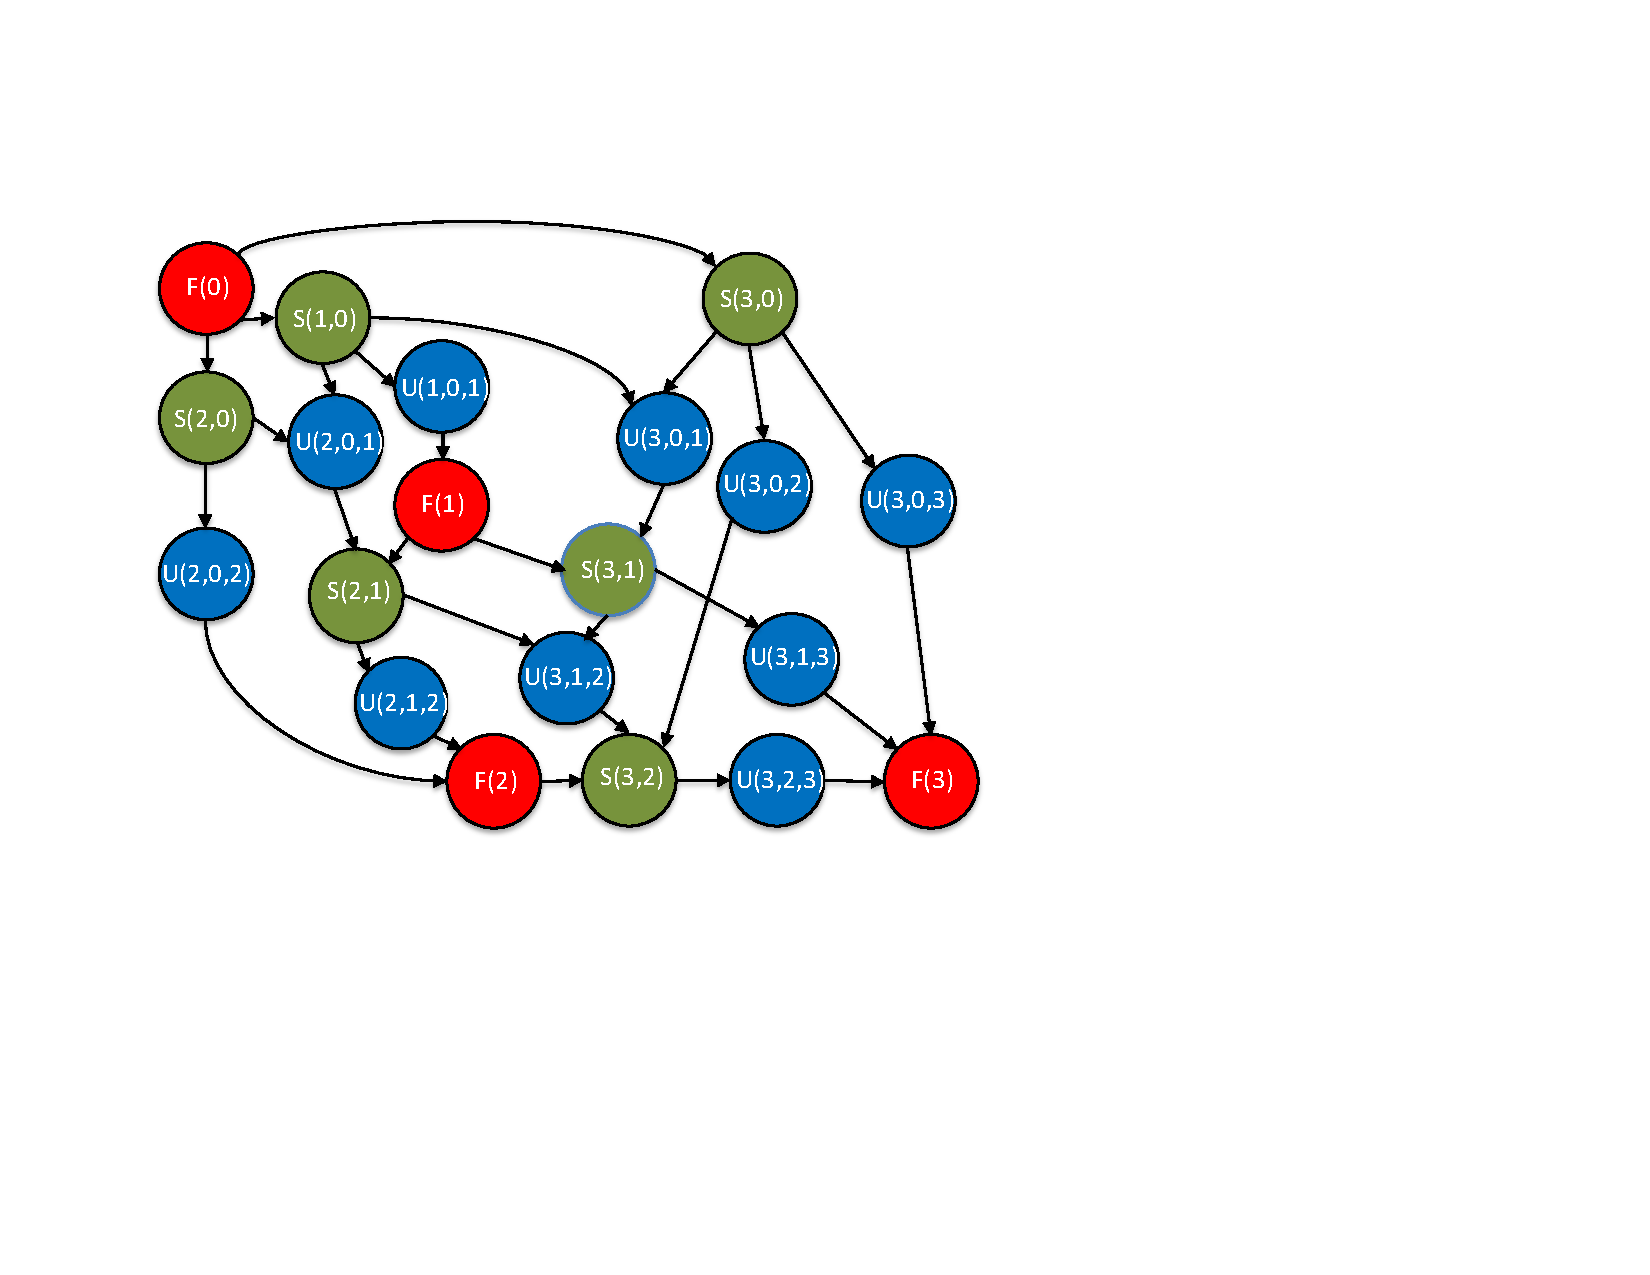
\includegraphics[width=.4\textwidth]{figures/cholesky.pdf}
\caption{Cholesky factorization DAG consisting of three types of tasks: F (Factor), S (Solve), U (update). Each task is associated with a partition of the input matrix called a {\em tile}. Arrows presesent data dependencies between tasks of different types or of the same task type but on different tiles. All data dependencies are called parcels.}
\label{fig:cholesky}
\end{figure}



\subsection{Defining a task}
RambutanAcc supports 3 types of task: (1) tasks running completely on the host, (2) tasks running on a group of accelerator cores, and (3) tasks running on host and offload kernels to the accelerator that comes along with host.
The first type supports computation on conventional processors (e.g. Intel's Ivy Bridge, AMD's Opteron, IBM's Power 8)  and many-core processor such as Intel's KNL.
The second type is for studying the benefit of fine-grained scheduling on a group of accelerator cores such as GPU's SM (Symmetric Multiprocessor), whereas the third type is useful when the programmer needs to retain legacy kernel code and study the communication among accelerators.
In the Cholesky factorization graph in Fig.~\ref{fig:cholesky}, it is reasonable to define {\em Factor} and {\em Solve} with the first type since they have low compute intensity. 
{\em Update}, on the contrary, should be defined to run on a group of accelerator cores (type 2) or on the whole accelerator (type 3).

For tasks running completely on the host (type 1), the process of defining a task includes the specification of data inputs and outputs, statements that the task will execute, and actions that should be performed upon completion of the task (e.g. create new tasks).
Defining inputs, outputs, and the post-completion action for tasks of type 2 and 3 are similar to type 1; however, the execution code for these two types is slightly different.
Specifically, the task code must be multithreaded and the abstract thread hierarchy for these tasks is very deep to support a substantially larger number of cores.
Fig.~\ref{fig:program} shows the kernel code of the {\em Update} task of sparse cholesky factorization, which is a sparse-sparse matrix multiply operation.
Like the CUDA programming model, each task kernel is executed by many threads (called a thread grid), organized into SIMD teams, each scheduled to run on a group of cores.
Teams scheduled (normally in a pipelined fashion) on the same group of cores are called thread blocks.
Type 3 tasks will invoke this kernel using a kernel launch interface (defined by hardware vendor such as NVIDIA) with many threads occupying the whole accelerator and hiding the latency from DRAM to registers.
For performance advantage, we expect the kernel launch to be asynchronous (though synchronous is fine for correctness).
The asynchronous launch returns a handle (e.g. a CUDA stream handle) and RambutanAcc only executes the post-completion action once this handle indicates that the kernel code on the accelerator has completed.
Unlike type 3, type 2 tasks do not have to spawn threads to occupy the whole accelerator.
RambutanAcc pre-spawns persistent kernels, and we utilize more threads than cores to hide the DRAM latency.
The task code is automatically offloaded to the accelerator by RambutanAcc's task scheduler.
No handle is needed in this case since RambutanAcc offloads the code and it is aware of when the code finishes.


\begin{figure}[htp]
\lstinputlisting[caption=]{code/example.c}
\caption{Kernel code of a task is executed by teams of threads. Each team is mapped to a group of accelerator cores and threads within the team are mapped to cores in the group. Teams mapped to the same group are called block. Note that for GPUs, each team should be a multiple of 16 SIMD threads to avoid thread divergence.}
\label{fig:program}
\end{figure}


\subsection{Execution model}
We next explain how the entire task dependency graph executes.
At the highest level, the graph is serviced by one or more processes, each consisting of one or more {\em workers}.
As previously mentioned, these workers can be CPU cores, accelerators, or groups of accelerator cores.
At the beginning, tasks that can run without any input dependencies are called {\em roots} of the graph, and they can be scheduled immediately.
In the task graph program described in Fig.~\ref{fig:cholesky}, task {\em F(0)} is the only root.
Once a root task finishes its execution, output data parcels may be produced.
Through the post-completion action, the task notifies the runtime about the availability of the data parcels so the runtime can create new tasks and transfer the parcels to where they are needed.
Note that the programmer has flexibility to control the location of newly created tasks, so task creation on a remote process is allowed.
As soon as the data required by a task has been fetched by the runtime, that task becomes runnable
and will be scheduled to execute on a worker.
The runtime scheduler periodically checks the availability of workers to schedule tasks.
A worker can be configured with a private task queue so that the scheduler can assign it new tasks even when the worker is already executing.
This capability allows tasks to be offloaded to workers on the accelerator at zero cost, since the time to move required data from host to accelerator can be overlapped with the execution of other tasks.

%A notable concern when programming on accelerators is that the DRAM capacity on accelerator is often modest compared to host DRAM.
%If this is the case, the programmer often decides to keep data on the host and stream only a portion of data to the accelerator at a time to compute before streaming the results back.
%Thus, if there are too many tasks created at the same location resulting in so much data being simultaneously fetched to that location, one may run out of memory.
%Since {\em RambutanAcc} allocates temporary buffers to perform the fetching work, it has the ability to maintain a reasonable amount of buffer to avoid this problem.


%\subsection{Example}
%Fig.~\ref{fig:firstProgram} presents some pseudo code to illustrate how a task can be defined to execute on the GPUs.
%Lines \#11 to \#17 show how a task registers with the runtime about inputs and outputs.
%In this case, a task depends on {\tt Unew} of the previous iteration and ghost cells of other tasks.
%The {\em dataMapping} function should swap {\tt Unew} and {\tt Old} for every iteration.
%All these data arrays reside in GPU DRAM.
%The {\em execute()} function offloads the function that will be executed and required arguments.
%System arguments such as thread and block indices are given by the runtime.


